% Author: Dominik Harmim <harmim6@gmail.com>

\documentclass[a4paper, 11pt, fleqn]{scrartcl}

\usepackage[czech]{babel}
\usepackage[utf8]{inputenc}
\usepackage[T1]{fontenc}
\usepackage{times}
\usepackage[left=2cm, top=3cm, text={17cm, 24cm}]{geometry}
\usepackage[unicode, colorlinks, hypertexnames=false, citecolor=red]{hyperref}
\usepackage{fancyhdr}
\usepackage{lastpage}
\usepackage[shortlabels]{enumitem}
\usepackage{amssymb}
\usepackage{amsmath}
\usepackage{newtxtext, newtxmath}
\usepackage{graphicx}

\newcommand{\NUMBER}{3}
\newcommand{\COURSE}{Teoretická informatika (TIN)}
\newcommand{\AUTHOR}{Dominik Harmim\,--\,xharmi00}

\newcommand*{\QEDB}{\hfill\ensuremath{\square}}

\pagestyle{fancy}
\fancyhead[L]{\AUTHOR}
\fancyhead[C]{\COURSE}
\fancyhead[R]{\today}

\fancyfoot[C]{}
\fancyfoot[R]{\thepage\,/\,\pageref*{LastPage}}

\setlength{\parindent}{0pt}
\setlength{\mathindent}{0pt}


\begin{document}
	\begin{center}
		{\Large Úkol~\NUMBER}
	\end{center}


	\section*{1.~příklad}

	Pomocí počátečních funkcí a~operátorů kombinace, kompozice a~primitivní
	rekurze vyjádřete funkci počítající odmocninu (zaokrouhlenou dolů na
	celá čísla):
	$$
		sqrt : \mathbb{N} \rightarrow \mathbb{N}, sqrt(x) = z\ \text{takové,
		že}\ z^2 \leq x \wedge (z + 1)^2 > x \text{.}
	$$
	Je možné použít funkce $ plus(x, y) $, $ mult(x, y) $, $ monus(x, y) $
	a~$ eq(x, y) $ definované v~přednáškách. Kromě nich však nepoužívejte
	žádné další funkce zavedené na přednáškách mimo funkce počáteční.
	Nepoužívejte zjednodušenou syntaxi zápisu funkcí\,--\,dodržte přesně
	definiční tvar operátorů kombinace, kompozice a~primitivní rekurze.

	\subsection*{Řešení:}

	\begin{align*}
		& rsqrt(x, 0) = \xi() \\
		& rsqrt(x, y + 1) = plus \circ (\pi^3_3(x, y, rsqrt(x, y)) \times
		(eq \circ ((monus \circ ((mult \circ (\pi^1_1(y) \times \pi^1_1(y)))
		\times \pi^1_1(x))) \times \xi()))) \\
		& \boldsymbol{sqrt} \equiv rsqrt \circ (\pi^1_1 \times \pi^1_1)
	\end{align*}


	\section*{2.~příklad}

	Mějme následující funkce:
	\begin{align*}
		& f(n) = \sqrt{2} n^3 \\
		& g(n) = 10\,000 n^2 + 500 n + 211 \text{.}
	\end{align*}
	Dokažte, že $ O(g(n)) \subset O(f(n)) $. \\
	\textbf{Pozn.:} Nezapomeňte, že důkaz má dvě části: (i)~$ O(g(n))
	\subseteq O(f(n)) $ a~(ii)~$ O(g(n)) \neq O(f(n)) $.

	\subsection*{Řešení:}

	\begin{itemize}
		\item
			S~využitím asymptotických odhadů složitosti můžeme říci, že
			$ O(f(n)) \approx O(n^3) $ a~$ O(g(n)) \approx O(n^2) $.

		\item
			Potom tedy budeme dokazovat ekvivalentní vztah $ \boldsymbol{
			O(g(n)) \subset O(f(n)) \Leftrightarrow O(n^2) \subset O(n^3)
			\Leftrightarrow (O(n^2) \subseteq} \boldsymbol{O(n^3) \wedge
			O(n^2) \neq O(n^3))} $.
	\end{itemize}
	Důkaz:
	\begin{enumerate}[(i)]
		\item
			Ukážeme, že $ \boldsymbol{O(n^2) \subseteq O(n^3)} $.

			\begin{itemize}
				\item
					Uvažme libovolné $ f(n) \in O(n^2) $.

				\item
					$ \exists c \in \mathbb{R}^+\ \exists n_0 \in
					\mathbb{N}\ \forall n \in \mathbb{N} : n \geq n_0
					\Rightarrow 0 \leq f(n) \leq c n^2 $.

				\item
					Zkoumejme nyní rychlost růstu~$ n^3 $ a~$ c n^2 $:
					\begin{align*}
						& \lim_{n\to\infty} \frac{n^3}{c n^2} =
						\begin{vmatrix}
							\lim\limits_{n\to\infty} n^3 = \infty \\
							\lim\limits_{n\to\infty} c n^2 = c \cdot \infty \\
							\text{lze užít L'Hospitalovo} \\ \text{pravidlo}
						\end{vmatrix} =
						\lim_{n\to\infty} \frac{3 n^2}{2 c n} =
						\begin{vmatrix}
							\lim\limits_{n\to\infty} 3 n^2 = \infty \\
							\lim\limits_{n\to\infty} 2 c n = c \cdot \infty \\
							\text{lze užít L'Hospitalovo} \\ \text{pravidlo}
						\end{vmatrix} =
						\lim_{n\to\infty} \frac{6 n}{2 c} = \frac{\infty}{
						\mathrm{sgn(c)}}
					\end{align*}

				\item
					$ n^3 $ tedy roste rychleji než~$ c n^2 $ a~musí tedy
					existovat $ n_0^\prime \in \mathbb{N} $ takové, že
					$ \forall n \in \mathbb{N} : n \geq n_0^\prime
					\Rightarrow 0 \leq f(n) \leq c n^2 \leq n^3 $. Tedy
					$ \forall n \in \mathbb{N} : n \geq n_0^\prime
					\Rightarrow f(n) \in O(n^2) $. Potom tedy \textbf{
					platí} $ \boldsymbol{O(n^2) \subseteq O(n^3)} $.
			\end{itemize}

		\item
			Ukažme, že $ \boldsymbol{O(n^2) \neq O(n^3)} $.

			\begin{itemize}
				\item
					Uvažme libovolné $ f(n) \in O(n^3) $.

				\item
					$ \exists c \in \mathbb{R}^+\ \exists n_0 \in
					\mathbb{N}\ \forall n \in \mathbb{N} : n \geq n_0
					\Rightarrow 0 \leq f(n) \leq c n^3 $.

				\item
					Zkoumejme nyní rychlost růstu~$ n^2 $ a~$ c n^3 $:
					\begin{align*}
						& \lim_{n\to\infty} \frac{n^2}{c n^3} =
						\begin{vmatrix}
							\lim\limits_{n\to\infty} n^2 = \infty \\
							\lim\limits_{n\to\infty} c n^3 = c \cdot \infty \\
							\text{lze užít L'Hospitalovo} \\ \text{pravidlo}
						\end{vmatrix} =
						\lim_{n\to\infty} \frac{2 n}{3 c n^2} =
						\begin{vmatrix}
							\lim\limits_{n\to\infty} 2 n = \infty \\
							\lim\limits_{n\to\infty} 3 c n^2 = c \cdot \infty \\
							\text{lze užít L'Hospitalovo} \\ \text{pravidlo}
						\end{vmatrix} =
						\lim_{n\to\infty} \frac{2}{6 c n} = 0
					\end{align*}

				\item
					$ n^2 $ tedy roste pomaleji než~$ c n^3 $ a~neexistuje
					tedy $ n_0^\prime \in \mathbb{N} $ takové, že $ \forall n
					\in \mathbb{N} : n \geq n_0^\prime \Rightarrow 0 \leq f(n)
					\leq c n^3 \leq n^2 $. Proto \textbf{neplatí} $ \boldsymbol{
					O(n^3) \subseteq O(n^2)} $. Z~toho plyne, že $ \boldsymbol{
					O(n^2) \neq O(n^3)} $.
			\end{itemize}

			\QEDB
	\end{enumerate}


	\section*{3.~příklad}

	Teta Květa stojí před regálem se zeleninou a~nehýbá se, protože má těžký
	rozhodovací problém. Potřebuje sníst co nejvíce vitamínu~C, aby ji přešla
	chřipka. Každý druh zeleniny je charakteristický obsahem vitamínu~C na
	kilo a~cenou za kilo. Teta se snaží přijít na to, jestli je možné nakoupit
	zeleninu za obnos~$ O $ v~její peněžence tak, aby úhrn vitamínu~C byl
	alespoň~$ C $. Kromě toho s~každým kilem zeleniny přidá zelinář deset deka
	brokolice zdarma, s~obsahem~$ B $ vitamínu~C na kilo.
	\medskip

	Formulujte problém tety Květy jako rozhodovací problém, a~dokažte, že je
	NP-úplný. Těžkost dokažte redukcí z~některého problému uvedeného v~odstavci
	\uv{NP-complete problems} zde: \\
	\url{https://en.wikipedia.org/wiki/NP-completeness\#NP-complete\_problems}
	\medskip

	Z~dálky na tetu volá synovec Alan, ať nezoufá, že to vyřeší za chvíli (tj.,
	v~polynomiálním čase), pomocí jakéhosi psacího stroje vlastní výroby
	s~nekonečnou páskou. Co to znamená pro lidstvo?

	\subsection*{Řešení:}

	\textbf{Formulace problému:}
	\begin{itemize}
		\item
			Problém tety Květy je možné charakterizovat jazykem $ K = \{
			z\,\#\,o\,\#\,c\ |\ o \in \mathbb{N} $ je obnos tety Květy v~její
			peněžence, za který nakupuje zeleninu; $ c \in \mathbb{N} $ je
			požadované minimální množství vitamínu~C; $ z $ je řetězec, který
			reprezentuje sekvenci dvojic $ \mathbb{N} \times \mathbb{N} $,
			kde prvky dvojic jsou odděleny např. znakem~$ @ $ a~jednotlivé
			dvojice jsou odděleny např. znakem~$ \$ $, každá dvojice
			reprezentuje kus zeleniny v~regálu, kde první složka dvojice
			představuje obsah vitamínu~C na kilo a~druhá složka představuje
			cenu na kilo daného druhu zeleniny, jednotlivé dvojice jsou
			číslovány např od~$ 0 \} $. Znak~$ \# $ je použit jako oddělovač.

		\item
			Aby byl v~této reprezentaci uvážen fakt, že s~každým kilem
			zeleniny dostane teta Květa deset deka brokolice zdarma
			s~obsahem $ B \in \mathbb{N} $ vitamínu~C na kilo, je k~první
			složce každé dvojice řetězce~$ z $ přičtena hodnota~$ \frac{B}{
			10} $ (tato hodnota je vhodně zaokrouhlena nebo jsou použita
			reálná čísla s~vhodným kódováním).

		\item
			Řešením tohoto problému je sekvence indexů kusů zeleniny
			z~řetězce~$ z $ taková, že suma cen vybraných kusů je menší nebo
			rovna dostupnému obnosu~$ o $ a~zároveň je suma množství
			vitamínu~C vybraných kusů větší nebo rovna požadovanému
			minimálnímu množství~$ c $.
	\end{itemize}

	\textbf{Důkaz NP-úplnosti:}
	\begin{enumerate}
		\item
			\textbf{Důkaz členství ve třídě NP:}

			\begin{itemize}
				\item
					Ukažme, že daný problém lze řešit nedeterministickým
					Turingovým strojem~$ M $ pracujícím v~polynomiálním
					čase.

				\item
					Zkonstruujeme~$ M $, který pro $ w \in K $ přijme
					v~polynomiálním čase.

					\begin{itemize}
						\item
							$ M $ ověří, zda jeho vstup je platná instance
							daného problému, tj. řetězec jazyka~$ K $.
							Pokud ne, odmítne. Toto lze ověřit
							v~čase~$ O(n) $.

						\item
							$ M $ nedeterministicky uhádne~$ k $ indexů
							kusů zeleniny na pomocnou pásku. Složitost
							tohoto kroku je~$ O(n) $.

						\item
							$ M $ ověří, zda vybrané index tvoří řešení
							daného problému, pokud ano, přijme, pokud ne,
							odmítne. Při tomto ověřování se budou sumy
							cen a~množství vitamínu~C zapisovat na další
							pomocnou pásku. Složitost bude~$ O(n^3) $.
					\end{itemize}

				\item
					$ M $ tedy pracuje v~polynomiálním čase.
			\end{itemize}

		\item
			\textbf{Důkaz NP-těžkosti:}

			\begin{itemize}
				\item
					Důkaz provedeme \textbf{polynomiální redukcí
					z~problému batohu (knapsack problem)}, který je
					NP-úplný.

				\item
					Problém batohu je definován následovně:

					\begin{itemize}
						\item
							Je dána konečná množina~$ R $, váhová
							funkce $ u : R \rightarrow \mathbb{N} $
							a~hodnotová funkce $ v : R \rightarrow
							\mathbb{N} $.

						\item
							Je dána mezní váha $ U \in \mathbb{N} $
							a~ mezní hodnota $ V \in \mathbb{N} $.

						\item
							Problém batohu se ptá, zda $ \exists
							R^\prime \subseteq R $ takové, že
							$ \sum\limits_{r \in R^\prime} u(r) \leq U
							\wedge \sum\limits_{r \in R^\prime} v(r)
							\geq V $.
					\end{itemize}

				\item
					Tuto redukci lze realizovat úplným deterministickým
					Turingovým strojem, který pracuje v~polynomiálním
					čas.

				\item
					Každou instanci problému batohu je možné převést
					na problém tety Květy následovně:

					\begin{itemize}
						\item
							Pro každý prvek množiny~$ R $ vytvoříme
							příslušnou dvojici v~řetězci~$ z $, kde
							první složka této dvojice bude dána
							hodnotovou funkcí~$ v $ ($ + \frac{B}{10} $
							za brokolici zdarma) a~druhá složka této
							dvojice bude dána váhovou funkcí~$ u $.

						\item
							Mezní váha~$ U $ bude zapsána do
							řetězce~$ o $. Mezní hodnota~$ V $ bude
							zapsána do řetězce~$ c $.

						\item
							Tímto vznikne řetězec jazyka~$ K $, tedy
							instance problému tety Květy.
					\end{itemize}
			\end{itemize}

			\QEDB
	\end{enumerate}

	\textbf{Co znamená pro lidstvo, že synovec Alan má stroj, který tento
	problém řeší v~polynomiálním čase?}
	\begin{itemize}
		\item
			Znamenalo by to, že existuje algoritmus, který tento problém
			řeší v~polynomiálním čase. To by znamenalo, že tento problém
			patří do třídy~P a~potom by muselo platit, že \textbf{P = NP}.

		\item
			Znamenalo by to, že každý problém, u~kterého dokáže počítač
			\uv{rychle} ověřit správnost řešení, dokáže počítač taky
			dané řešení \uv{rychle} nalézt.
	\end{itemize}


	\section*{4.~příklad}

	Modelujte následující kritický systém Petriho sítí. Namalujte ji
	a~zapište formálně ve shodě s~definicí.
	\medskip

	Převozník chce převézt z~jednoho břehu na druhý hlávku zelí, kozu
	a~vlka. Do loďky s~sebou může vzít buď zelí, nebo kozu, nebo
	vlka, ale víc se tam nevejde. Nechá-li na břehu hlávku zelí
	a~kozu, koza zelí sežere. Nechá-li na břehu kozu a~vlka, pak
	vlk sežere kozu. Jakým způsobem musí převozník postupovat, aby
	nedošlo k~žádné škodě?
	\medskip

	Snažte se o~přehlednost a~pochopitelnost modelu. Místa vhodně
	pojmenujte a~síť nakreslete přehledně. (příklad ze sbírky úloh
	Alkuina z~Yorku, Úlohy k~bystření mladíků, z~roku cca 735-804)

	\subsection*{Řešení:}

	\textbf{Grafická reprezentace Petriho sítě:}
	\begin{center}
		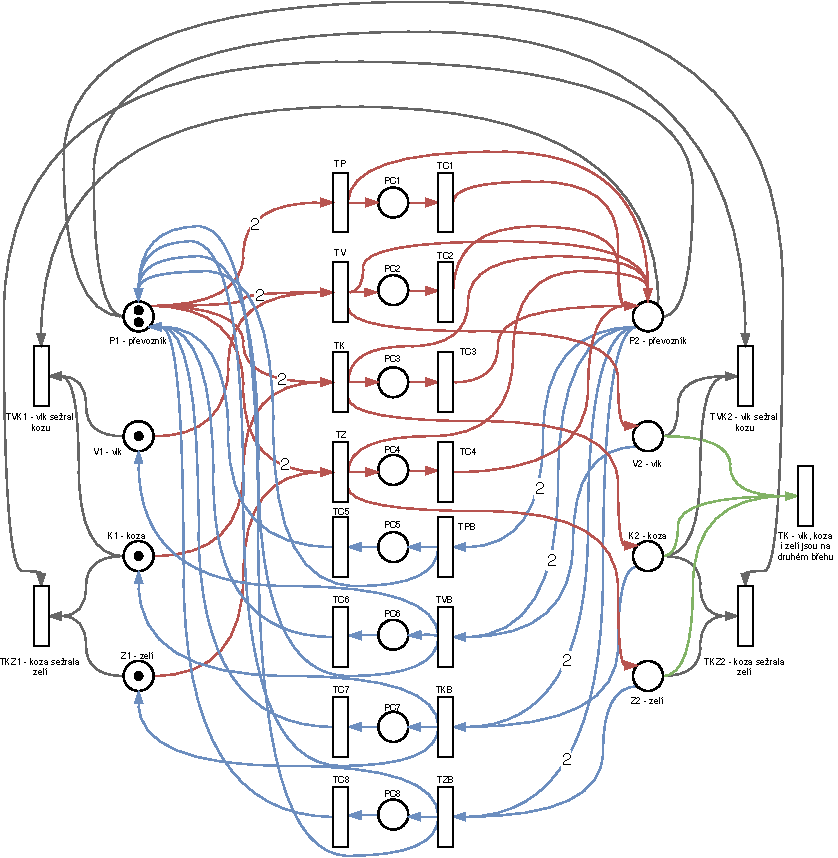
\includegraphics[width=.95 \linewidth]{img/pt.pdf}
	\end{center}

	\textbf{Formální zápis Petriho sítě:} \\
	$ N = (P, T, F, W, K, M_0) $, kde
	\begin{itemize}
		\item
			$ P = \{P1, V1, K1, Z1, P2, K2, Z2, PC1, PC2, PC3,
			PC4, PC5, PC6, PC7, PC8\} $

		\item
			$ T = \{TVK1, TKZ1, TVK2, TKZ2, TK, TC1, TC2, TC3,
			TC4, TC5, TC6, TC7, TC8, TP, TV, TK, TZ, \\ TPB, TVB,
			TKB, TZB\} $

		\item
			$ F = \{(P1, TP), (P1, TV), (P1, TK), (P1, TZ),
			(P1, TVK2), (P1, TKZ2), (P2, TPB), (P2, TVB),
			(P2, TKB), \\ (P2, TZB), (P2, TVK1), (P1, TKZ1),
			(V1, TV), (V1, TVK1), (V2, TVB), (V2, TVK2),
			(K1, TK), \\ (K1, TVK1), (K1, TKZ1), (K2, TKB),
			(K2, TVK2), (K2, TKZ2), (Z1, TZ), (Z1, TKZ1),
			(Z2, TZB), \\ (Z2, TKZ2), (PC1, TC1), (PC2, TC2),
			(PC3, TC3), (PC4, TC4), (PC5, TC5), (PC6, TC6),
			(PC7, TC7), \\ (PC8, TC8), (TC1, P2), (TC2, P2),
			(TC3, P2), (TC4, P2), (TC5, P1), (TC6, P1),
			(TC7, P1), (TC8, P1), \\ (V2, TK), (K2, TK),
			(Z2, TK), (TP, PC1), (TP, P2), (TV, PC2),
			(TV, P2), (TV, V2), (TK, PC3), (TK, P2), \\
			(TK, K2), (TZ, PC4), (TZ, P2), (TZ, Z2),
			(TVB, PC6), (TVB, P1), (TVB, V1), (TPB, PC5),
			(TPB, P1), \\ (TKB, PC7), (TKB, P1), (TKB, K1),
			(TZB, PC8), (TZB, P1), (TZB, Z1)\} $

		\item
			$ W =
				\begin{cases}
					2 & \text{pro}\ (P1, TP) \\
					2 & \text{pro}\ (P1, TV) \\
					2 & \text{pro}\ (P1, TK) \\
					2 & \text{pro}\ (P1, TZ) \\
					2 & \text{pro}\ (P2, TPB) \\
					2 & \text{pro}\ (P2, TVB) \\
					2 & \text{pro}\ (P2, TKB) \\
					2 & \text{pro}\ (P2, TZB) \\
					1 & \text{jinak}
				\end{cases}
			$

		\item
			$ K =
				\begin{cases}
					2 & \text{pro}\ P1 \\
					2 & \text{pro}\ P2 \\
					1 & \text{jinak}
				\end{cases}
			$

		\item
			$ M_0 =
				\begin{cases}
					2 & \text{pro}\ P1 \\
					1 & \text{pro}\ V1 \\
					1 & \text{pro}\ K1 \\
					1 & \text{pro}\ Z1 \\
					0 & \text{jinak}
				\end{cases}
			$
	\end{itemize}
\end{document}
